\chapter{Modelo de Jaynes-Cummings}
\label{ch3_jcm}

%CAMBIAR ESTO PARA PERSONALIZARLO A MI GUSTO
\pagestyle{fancy}
\fancyhf{}
\fancyhead[LE]{\nouppercase{\rightmark\hfill}}
\fancyhead[RO]{\nouppercase{\leftmark\hfill}}
\fancyfoot[LE,RO]{\hfill\thepage\hfill}

En este capitulo analizaremos en profundidad la din\'amica y los aspectos teoricos mas importantes 
del modelo de Jaynes-Cummings, abordando el problema tanto desde un lado te\'orico, como desde
el lado computacional, necesario para resolver la din\'amica en sistemas abiertos.
Primero se trabajar\'a en el modelo de un átomo en una cavidad, se analizar\'an los casos importantes,
y se explicar\' la din\'amica del problema. Esto es importante para comprender conceptualmente como
interact\'uan fundamentalmente la materia y la luz, y nos sirve para conseguir buena intuici\'on del
problema de dos átomos. Tambien se ver\'a la influencia del entorno sobre la cavidad, permitiendo
perdida (o absorci\'on) de fotones, y tambien el bombeo coherente que puede excitar espontaneamente
al átomo. \newline

\section{Modelo y aproximaciónes}
Comencemos entonces por el paradigmatico modelo de 1 átomo. El modelo de Jaynes-Cummings consiste en describir la interacción entre la materia y la luz de manera cuantica, y el experimento mas sencillo consta de un átomo de dos niveles atrapada en una cavidad. La simpleza del modelo surge de las aproximaciónes e hipotesis que se hacen, en primer lugar, el campo electromagnetico dentro de la cavidad puede en principio tener infinitos modos, pero para simplificar se considera solo un modo. 
Entonces tenemos un Hamiltoniano ($\hbar = 1$)

\begin{equation}\label{eq3:hamiltoniano inicial}
\begin{aligned}
    \hat H & = \hat H_A + \hat H_C + \hat H_{int}  \\
    \hat H_A &= \omega \frac{\sigma_z}{2} \\
    \hat H_C &= \epsilon \hat a^\dagger\hat a = \epsilon \hat n \\
    \hat H_{int} &= -i g (\hat\sigma_-+\hat \sigma_+)(\hat a - \hat a^\dagger)
\end{aligned}
\end{equation}
donde $\epsilon$ y $\omega$ son las freccuencias naturales de la cavidad y del átomo respctivamente. Los operadores $\hat a$ y $\hat a^\dagger$ son los operadores de aniquilaci\'on y creaci\'on fot\'onicos de la cavidad y $\hat n =a^\dagger a$ es el operador de n\'umero de la cavidad, y $\hat \sigma_z$ es el operador de pauli. Los estados del átomo de dos niveles los llamamos $\ket{g}$ y $\ket{e}$ al estado ground y excitado respectivamente, y con esta notación los operadores $\sigma_\pm = (\sigma_x\pm i\sigma_y)/2$ son los operadores de subida y bajada atomicos. 
La interacci\'on es complicada, y para simplificar lo que se hace es usar la representaci\'on de interacci\'on, y uno encuentra que hay dos frecuencias, una que llamamos \textit{rotante} y es la diferencia entre las frecuencias caracteristicas $\epsilon-\omega$, y la otra frecuencia es la suma $\epsilon+\omega$. La aproximación de onda rotante vale cuando las frecuencias son similares $\epsilon\sim\omega$, y consta de despreciar la dinamica de los terminos contrarrotantes, ya que oscilan muy rapidamente en comparación con los terminos rotantes, y entonces podemos promediar los efectos de los terminos rapidos. Entonces al aplicar esta aproximación, justificada cuando $\epsilon\sim\omega$ y $g \ll \epsilon,\omega$ se obtiene el hamiltoniano de JC \ref{}\textcolor{red}{ludmi 49}
\begin{equation}
    H_{JC}=\epsilon a^\dagger a + \omega \sigma_z/2 + g(a^\dagger\sigma_-+a\sigma_+)
\end{equation} 
La interpretaci\'on de la interacci\'on en este caso es clara, las dos opciones son que el átomo suba un nivel de energ\'ia y en consecuencia la cavidad pierda un fot\'on, o que el átomo baje un nivel, y la cavidad gane una excitaci\'on. Este Hamiltoniano conserva el n\'umero total de excitaciones $\hat N= \hat n + \hat \sigma$. En este momento es usual aplicar una transformación unitaria $K=\exp{-i\omega t(a ^\dagger a + \sigma_z/2)}$ sobre el Hamiltoniano que queda 
\begin{equation}\label{eq3:hamiltoniano jcm}
    H=\frac{\Delta}{2}\sigma_z+g(a^\dagger \sigma_-+a \sigma_+)
\end{equation}
donde $\Delta = \epsilon - \omega$ es el \textit{detunning} entre las frecuencias de la cavidad y el átomo. Un ejemplo de esto es un átomo de Rydberg metido en una cavidad \ref{}, o ... \textcolor{red}{BUSCAR EJEMPLOS}.
Como el Hamiltoniano conserva la cantidad de excitaciones es oportuno agrupar los estados en funci\'on de la cantidad de excitaciones: $\{\ket{g,n},\ket{e,n-1}\}$. En esta base el Hamiltoniano se diagonaliza por bloques, ya que las interacciones conservan la cantidad total de excitaciones, entonces los elementos de matriz entre estados con diferente cantidad de excitaciones se corresponde
\begin{align*}
    [H,\hat N]=0 \implies & \bra{N'}H \hat N \ket{N} = \bra{N'}\hat N H \ket{N} \\
    & N \bra{N'}H  \ket{N} = N' \bra{N'}H \ket{N} \\
    & \implies \bra{N'}H \ket{N} = \begin{cases}
        0 \text{ , si } N' \neq N \\
        \bra{N}H \ket{N} \text{ , si } N'=N
    \end{cases}
\end{align*}
donde $\ket{N}$ es un estado con $N$ excitaciones totales. Entonces para resolver el problema solo tenemos que mirar el subespacio de 2x2 de n excitaciones, cuyo Hamiltoniano es
\begin{equation}
    H_n=\begin{pmatrix}
        -\frac{\Delta}{2} & g \sqrt{n} \\
        g \sqrt{n} & \frac{\Delta}{2} 
    \end{pmatrix}
\end{equation}
Resolvemos el problema de autovalores y autovectores y obtenemos
\begin{equation}
    \begin{aligned}
        \ket{\psi^n_-} & = \cos \frac{\theta_n}{2}\ket{g,n}-\sin \frac{\theta_n}{2}\ket{e,n-1} \\
        \ket{\psi^n_+} & = \sin \frac{\theta_n}{2}\ket{g,n}+\cos \frac{\theta_n}{2}\ket{e,n-1}        
    \end{aligned}
\end{equation}
con $E_{\pm}^n=\pm \frac{\Omega_n}{2}$ las autoenergias y $\Omega_n=\sqrt{\Delta^2+4g^2n}$ la frecuencia de Rabi del sistema, $\cos \theta_n=\frac{\Delta}{\Omega_n}$ modulando la superposici\'on de estados. 
\begin{figure}
    \centering
    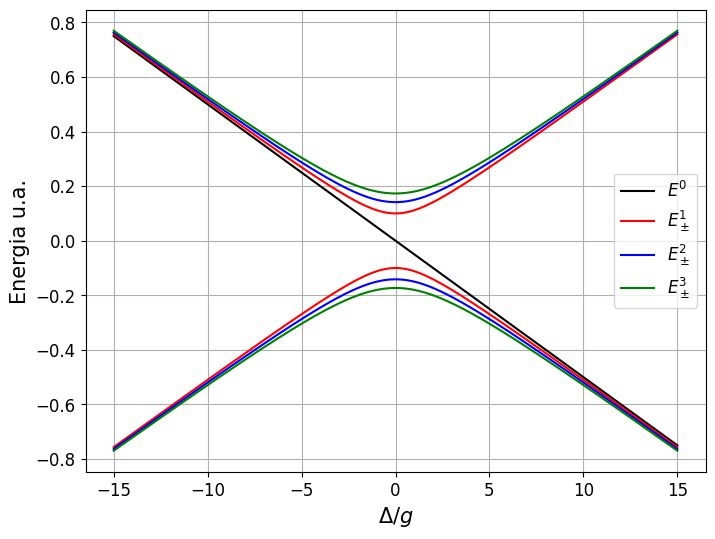
\includegraphics[width=0.7\textwidth]{figuras/ch3/relacion energia detunning jcm simple.png}
    \caption{Relaci\'on energ\'ia detunning para el modelo de Jaynes-Cummings. La diferencia de energ\'ia entre los estados de un mismo nivel para $\Delta=0$ es $2g\sqrt{n}$.}
    \label{fig:relación energia detunning jcm1}
\end{figure}
En la figura \ref{fig:relación energia detunning jcm1} se observan las curvas de energ\'ia en funci\'on del detunning para diferentes niveles. Lo primero que tenemos que observar es que en el caso resonante, es decir $\Delta=0$, los autoestados del sistema son los estados maximamente entrelazados de Bell
\begin{equation}
    \ket{\psi_\pm^n}=\frac{1}{\sqrt{2}}(\ket{gn}\pm\ket{e,n-1})
\end{equation} 
y la diferencia de energ\'ia entre los autoestados es $\Delta E^n =E^n_+-E^n_-=2g\sqrt{n}$. En el caso muy lejos de resonancia podemos asumir que $\Delta \gg g $, y entonces los autoestados coinciden en este l\'imite con los estados de la base, 
\begin{equation}
    \begin{aligned}
        \ket{\psi^n_+}=\ket{e,n-1} \\
        \ket{\psi^n_-}=\ket{g,n}
    \end{aligned}
\end{equation}
Ac\'a hay una sutileza, y es que si $\Delta>0$, entonces $\ket{e,n-1}$ es el estado de mayor energ\'ia y la notaci\'on coincide con la energ\'ia, pero si $\Delta<0$ entonces el estado $\ket{\psi^n_+}$ es el estado de menor energ\'ia. 
Un efecto interesante es que en el caso de alta desinton\'ia, podemos calcular la diferencia entre la energía del autoestado exacto del Hamiltoniano $\ket{\psi_\pm^n}$ y la energía asintotica a la que tiende, que es la energía de los estados de la base $\ket{g,n},\ket{e,n-1}$. Esta diferencia ... \textcolor{red}{VOLVER A ESTO Y VER SI DEJARLO O SACARLO. EVENTUALMENTE COMPLETAR.}
\begin{equation}
    \begin{aligned}
        \Delta E_{e,n-1}=E_+^n-E^{(0)}_{e,n-1}=\frac{g^2}{\Delta}n
        \Delta E_{g,n}=E_-^n-E^{(0)}_{g,n}=-\frac{g^2}{\Delta}n
    \end{aligned}
\end{equation}
El resultado importante de esta diferencia de energias es que aun en ausencia de fotones en la cavidad $n=0$, hay una diferencia entre las energias entre el Hamiltoniano del átomo, y del $H_{JC}$. Este efecto es el \textit{Lamb Shift} y nos dice que el vac\'io electromagnetico induce un corrimiento en la energ\'ia de los estados. Esto es importante notarlo, porque para el caso de dos átomos tambien est\'a manifiesto.

\subsection{Fase geométrica en el JCM}
Vamos a analizar la fase de Berry y la fase geométrica en la aproximación cinemática.
\subsubsection{Fase de Berry}
Para ver la fase de berry tenemos que tener un parámetro de control en el Hamiltoniano, el cual varía lentamente. Para esto necesitamos aplicar una transformación unitaria de corrimiento de fase al Hamiltoniano original \ref{eq3:hamiltoniano jcm} $R=\exp{-i\Omega a^\dagger a}$, que queda
\begin{equation}
    H=\frac{\Delta}{2}\sigma_z+g(a^\dagger \sigma_e^{-i\Omega}-+a\sigma_+e^{i\Omega})
\end{equation}
que ahora depende explicitamente del parámetro externo de control $\Omega$. Los autoestados de este nuevo Hamiltoniano se obtienen aplicando esta misma transformación sobre los autoestados del Hamiltoniano original. Si el parámetro de control varia lentamente entre 0 y $2\pi$, entonces estamos dentro de las hipotesis propuestas por Berry, y podemos calcular la fase de Berry mediante la ecuación \ref{eq2:fg berry}:
\begin{equation}
    \psi_a^n=i\oint_Cd\Omega\bra{\psi_\pm^n}R(\Omega)^\dagger \frac{d}{d\Omega}\ket{\psi_\pm^n}=\pi(1\pm \cos(\theta_n))
\end{equation}

que es no trivial incluso para $n=0$, lo que nos dice que incluso el vacio electromagnetico introduce una corrección en la fase de Berry.
\subsubsection{Aproximación Cinemática}
Para comparar ambos metodos, ahora vamos a calcular la fase geométrica utilizando la aproximación cinemática aunque este abordaje es más general de lo necesario en este caso.
Si se considera que el estado inicial es un atuoestado del Hamiltoniano, como los estados $\ket{\psi_\pm^n}$, entonces la fase geométrica en este caso se anula. Pero si se considera un estado inicial, por ejemplo $\ket{\psi(0)}=\ket{e,n}$, entonces el estado a tiempo $t$ resulta
\begin{equation}\label{eq3:fg berry jcm}
    \ket{\psi(t)}=(\cos^2\theta_ne^{-iE_+^nt}+\sin^2\theta_ne^{iE_+^nt})\ket{e,n}-i \sin\theta_n\sin(E_+^nt)\ket{g,n+1}
\end{equation}
La fase geometrica acumulada \ref{eq2:fg cinematica unitaria} es
\begin{equation}\label{eq3:fg unitaria jcm}
    \phi_u[C]=-\pi(1-\cos\theta_n)\frac{t}{T} +\arg\left\{ 1+e^{2\pi i \frac{t}{T}}\frac{\Omega_n-\Delta}{\Omega_n+\Delta} \right\}
\end{equation}
con $T=\frac{2\pi}{\Omega_n}$ es un período correspondiente a la frecuencia de Rabi $\Omega_n$. Esta expresión y la antrior \ref{eq3:fg berry jcm}, deberian coincidir cuando $t=T$, que se corresponde con un ciclo cerrado. En este caso ($t=T$) se obtiene
\begin{equation}
    \phi_u=-\pi(1-\cos\theta_n)
\end{equation}
La diferencia de signos se puede explicar comparando las curvas descritas por la esfera de Bloch para cada evolución. 
\begin{figure}[H]
    \centering
    \begin{subfigure}[h]{0.49\textwidth}
        \centering
        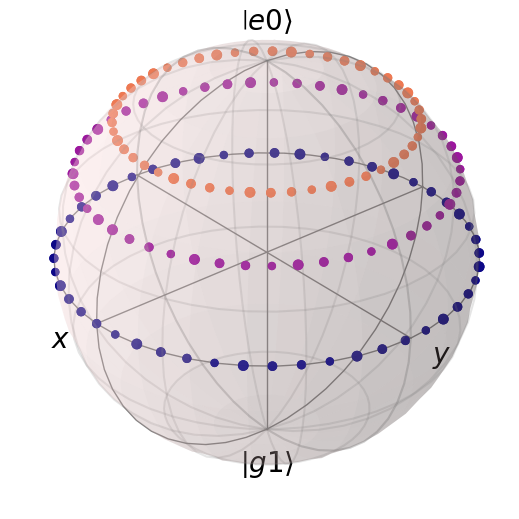
\includegraphics[width=\textwidth]{figuras/ch3/bloch berry.png}
        \caption{Evolución adiabática} 
        \label{fig3:bloch berry}
    \end{subfigure}
    \hfill
    \begin{subfigure}[h]{0.49\textwidth}
        \centering
        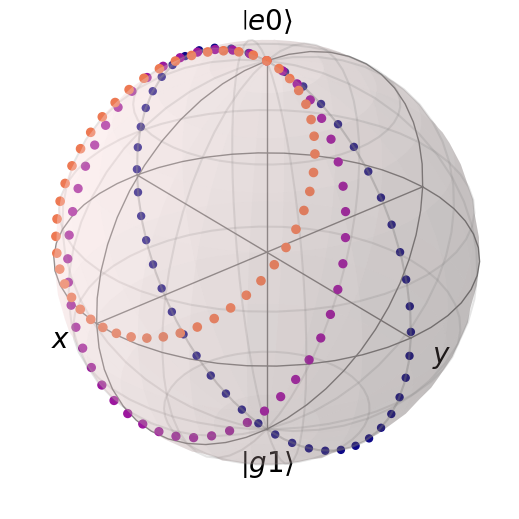
\includegraphics[width=\textwidth]{figuras/ch3/bloch cinematica.png}
        \caption{Enfoque cinemático}
        \label{fig3:bloch cinematica}
    \end{subfigure}
    \caption{}
    \label{fig3:esfera de bloch jcm}
\end{figure}
En el caso \ref{eq3:fg berry jcm}, correspondiente a la figura \ref{fig3:bloch berry}, los autoestados son los autoestados $R(\Omega)\ket{\psi_\pm^n}=e^{-i\Omega \hat n}\ket{\psi_\pm^n}$, entonces al variar $\Omega\in [0,2\pi]$ la trayectoria es simplemente un circulo en la esfera de Bloch. En cambio, en el segundo caso, si preparamos el sistema inicialmente en el estado $\ket{e,n}$ y lo dejamos evolucionar por la acción de H durante un tiempo, la trayectoria ahora no son circulos horizontales en la esfera, sino que parten del polo norte, que es el estado $\ket{e,n}$, y luego hace una trayectoria ovalada, para finalmente volver al punto inicial de partida a un tiempo $t=T$. La diferencia en el signo se explica a travez de la transformación que nos lleva de una curva a la otra. Para esto, necesitamos de una rotacion rigida, y una inversion de la parametrizacion, por su parte, esta ultima, introduce un signo negativo, cosa que se ve claramente en la ecuacion \ref{eq3:fg unitaria jcm} al cambiar $t\rightarrow -t$.

\textcolor{red}{aca puedo intentar de agregar el caso con medio kerr. Creo que no es tan complicado y el problema de autocosas ya lo tengo medio resuelto en papel desde hace un tiempo, pero lo tengo que revisar a ver si esta bien y lo tengo que completar, pero puede estar bueno para entender que le hace a la FG desde el vamos.}

\section{Medio Kerr}\label{sec3:medio kerr}
Ahora que ya se trabajó el caso mas sencillo, se comienza a estudiar casos mas generales. La primera generalización que se hará es agregar un medio no lineal. Este medio se lo conoce como medio Kerr, y lo que hace es agregar un término en el Hamiltoniano de la cavidad, que pasa de ser \ref{eq3:hamiltoniano inicial} 
\begin{equation}
    H_C=\epsilon \hat n \rightarrow H_C^{\text{Kerr}}=\epsilon \hat n (1-\frac{\chi}{\epsilon})
\end{equation}
donde $\chi$ es el parámetro que caracteriza al medio de la cavidad Kerr. Si se realizan nuevamente los mismos pasos, se arriba a las mismas conclusiones sobre la forma del Hamiltoniano, y se tiene que 
\begin{equation}
    H=\frac{\Delta}{2}\hat \sigma_z+\chi \hat n^2+g(\hat a^\dagger \hat \sigma_-\hat a \hat \sigma_+)
\end{equation}
y en forma matricial, en el subespacio de n excitaciones $\{\ket{gn},\ket{e,n-1}\}$
\begin{equation}
    H^{(n)} = \begin{pmatrix}
        -\frac{\Delta}{2}+\chi n^2 & g \sqrt{n} \\
        g \sqrt{n} & \frac{\Delta}{2}+\chi (n-1)^2 
    \end{pmatrix}
\end{equation}
Resolviendo, se obtiene que ahora los autovectores son
\begin{equation}
    \ket{\psi_\pm^n}=\frac{1}{N_\pm} \left( (-\frac{\Delta}{2}+\chi(n-1/2)\mp\frac{\Omega_{n,\chi}}{2}) \ket{gn} + g\sqrt{n} \ket{e,n-1}  \right)
\end{equation}
donde $\Omega_{n,\chi}=\sqrt{(\chi(n-1/2)-\Delta)^2+4g^2n}$, $N_\pm=\sqrt{(-\frac{\Delta}{2}+\chi(n-1/2)\mp\Omega_{n,\chi}/2)^2+g^2n}$, y las autoenergias son 
\begin{equation}\label{eq3:autoenergia kerr}
    E_\pm^n=\chi(n-\frac{1}{2})^2 +\frac{\chi}{4} \pm \frac{\Omega_{n,\chi}}{2}
\end{equation}
Se puede ver que el resultado con $\chi=0$ se reduce al caso visto anteriormente, que representa una cavidad con un medio lineal.

Si uno quiere resolver la dinamica de este problema para un estado inicial cualquiera, lo que tenemos que hacer es desarrollar este estado inicial en funcion de los autoestados del problema, entonces tendriamos para un estado arbitrario con un numero total de excitaciones definido, que suponemos igual a 1 por simplificacion (la generalizacion es inmediata):
\begin{equation}
    \ket{\psi}(t)=U(t)(\braket{\psi_+^1}{\psi(0)}\ket{\psi_+^1}+\braket{\psi_-^1}{\psi(0)}\ket{\psi_-^1})=c_+e^{-iE_+t}\ket{\psi_+}+c_-e^{-iE_-t}\ket{\psi_-}
\end{equation}
Lo interesante de esto es que podemos sacar de factor comun alguna de las dos energias, y entonces lo importante para la evolucion temporal del sistema es la diferencia entre las energias, por lo tanto, la cantidad relevante sigue siendo $\Omega_{n,\chi}$, que es la frecuencia de Rabi para medios tipo Kerr. Por otro lado, el producto interno que da lugar a los coeficientes $c_\pm$ depende de $\chi$, por lo tanto las amplitudes de probabilidad de encontrar al estado temporalmente evolucionado en algun otro estado haciendo una medicion proyectiva, depende de $\chi$. Por lo tanto, se puede decir que el medio Kerr modifica las amplitudes de oscilacion de las poblaciones del estado.

Entonces se analiza la relacion entre $\pm \Omega_{n,\chi}/2$ y el detunning, tienendo en cuenta que ahora el medio puede tener $\chi \neq 0$. 

\begin{figure}[H]
    \centering
    \begin{subfigure}[h]{0.49\textwidth}
        \centering
        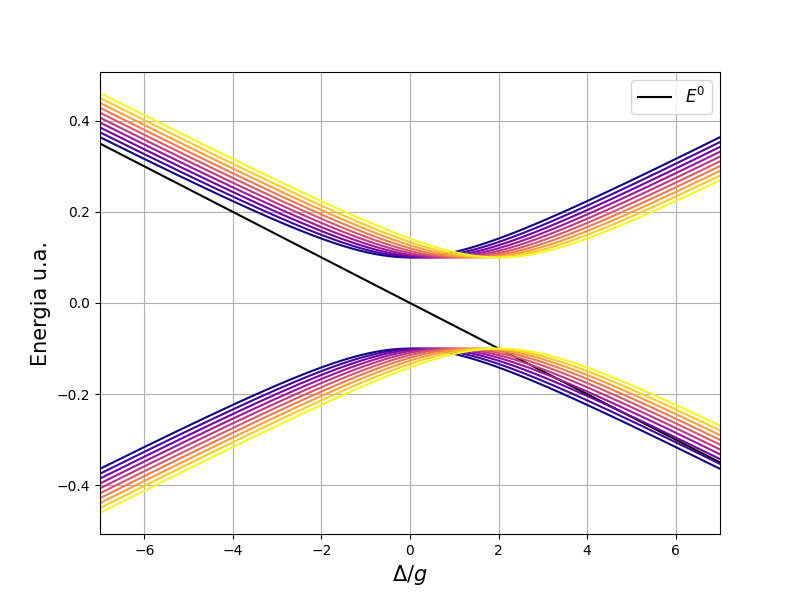
\includegraphics[width=\textwidth]{figuras/ch3/relacion energia detunning jcm simple kerr.png}
        \caption{N=1}
        \label{fig3:relacion energia detunning kerr 1}
    \end{subfigure}
    \hfill
    \begin{subfigure}[h]{0.49\textwidth}
        \centering
        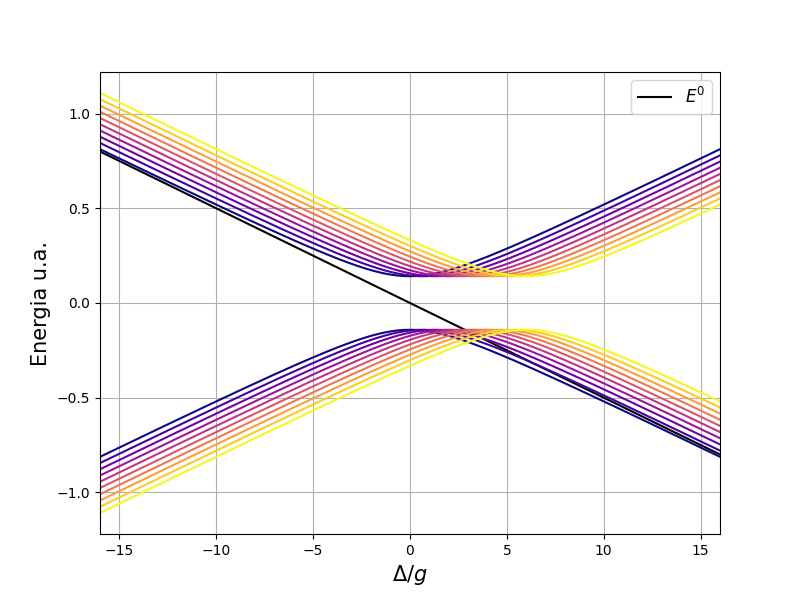
\includegraphics[width=\textwidth]{figuras/ch3/relacion energia detunning jcm simple kerr 2.png}
        \caption{N=3}
        \label{fig3:relacion energia detunning kerr 2}
    \end{subfigure}
    \caption{Grafico de la frecuencia de Rabi $\Omega_{N,\chi}$ en funcion del detunning $\Delta$ para N=1 y N=3.}
    \label{fig3:relacion energia detunning kerr}
\end{figure}

Se observa en la figura \ref{fig3:relacion energia detunning kerr} las diferencias entre autoenergias van cambiando para diferentes valores de $\chi$, donde en el panel \ref{fig3:relacion energia detunning kerr 1} se observa las energias para N=1 y en \ref{fig3:relacion energia detunning kerr 2} para N=3, en función del detunning, y en colores se ve de mas oscuro a mas claro, como el aumento de $\chi \in [0,2g]$ afecta a las curvas. Lo que se observa es que, al aumentar $\chi$, las curvas se desplazan hacia la derecha en una cantidad $\chi(n-1/2)$. 

Este comportamiento se puede predecir mirando la forma de la autoenergia \ref{eq3:autoenergia kerr}, ya que lo que estamos haciendo es desplazando la raiz haciendo un cambio de variables $\Delta \rightarrow \Delta - \chi(n-1/2)$. Este desplazamiento depende del número de excitaciones N. 
Dados dos valores diferentes de $\chi$ nos interesa saber si al aumentar $\Delta$, aumenta o disminuye las energias de los estados, para esto buscamos la interseccion entre dos curvas con diferentes $\chi$, que llamamos $\chi_1$ y $\chi_2$, con $\chi_1<\chi_2$. Haciendo el calculo obtenemos que la interseccion es para $\Delta=(2n-1)\frac{\chi_1+\chi_2}{2}$, es decir, si $\Delta<(2n-1)\frac{\chi_1+\chi_2}{2}$ entonces la frecuencia de $\chi_2$ es mayor que la de $\chi_1$ y por lo tanto oscila mas rapidamente, y viceversa si $\Delta>(2n-1)\frac{\chi_1+\chi_2}{2}$.

Ahora, habiendo entendido esto, podemos ver que el efecto del medio es modificar la frecuencia y tambien la amplitud de la oscilacion, haciendo que la primera sea menor, y \textcolor{red}{para ver que pasa con las amplitudes tengo que hacer algunas cuentas}


\section{JCM disipativo}


Habiendo desarrollado el análisis de la fase geométrica acumulada por el sistema átomo-cavidad en la situación ideal de completo aislamiento, se aborda ahora el estudio para el escenario más realista en el que el mismo sistema se encuentra en interacción con un entorno. El problema se trata para la implementación específica en estructuras semiconductoras, en las que un punto cuántico (al cual se sigue, sin embargo, refiriendo como átomo o sistema de dos niveles) se ubica en una nano o micro-cavidad.

Siguiendo \cite{80}, en este capítulo se estudia en detalle la fase geométrica acumulada en un modelo de Jaynes-Cummings disipativo, como caso paradigmático dentro del campo de la electrodinámica en cavidades. Se considera que los principales mecanismos por los cuales el sistema “átomo + modo” interactúa con el entorno son el flujo de fotones a través de las paredes de la cavidad y el continuo e incoherente bombeo del sistema de dos niveles, lo que conforma un escenario frecuente en electrodinámica de cavidades semiconductoras \cite{81,82,83}. 

Para poder modelar estos mecanismos, se emplea la ecuación maestra fenomenológica de Lindblad
\begin{equation}\label{eq3:lindblad}
\dot{\rho}(t) = -i [H, \rho(t)] + \frac{1}{2} \sum_\alpha \big( 2L_\alpha \rho(t) L_\alpha^{\dagger} - \{ L_\alpha^{\dagger}L_\alpha, \rho(t) \} \big),
\end{equation}

, despreciando otros procesos con menor influencia en la dinámica como el desfasaje puro o el bombeo de fotones del entorno en la cavidad, considerando además que el entorno se halla a temperatura cero. Los operadores de Lindblad

\begin{equation}
L_\gamma = \sqrt{\gamma} \ a
\end{equation}
\begin{equation}
L_p = \sqrt{p} \ \sigma_+
\end{equation}

,representan la pérdida de fotones y el bombeo continuo e incoherente del átomo, respectivamente, con los parámetros $\gamma$ y $p$ denominados tasa de pérdida de fotones y amplitud del bombeo. 

El bombeo sobre el átomo es siempre secundario frente a la pérdida de fotones, lo cual nos da las relaciones $\frac{p}{g},\frac{p}{\gamma} \ll 1$, y la relación entre $\gamma$ y $g$ da lugar a dos regimenes que se diferencian con claridad \cite{50}-\cite{54}. El regimen de acoplamiento fuerte (SC o Strong Coupling) es cuando la interacción átomo-cavidad es mas fuerte que la disipación del entorno, es decir $\gamma /g <1$. En el caso contrario $\gamma/g>1$ estamos en el régimen de acoplamiento débil (WC o Weak Coupling). Para no generar confusiones, hay que destacar que en general, cuando en la literatura se habla de acoplamientos fuertes y debiles, se refiere a la interacción entre las partes del mismo sistema, pero en este caso, se esta haciendo referencia a la interacción del sistema con el entorno EN COMPARACIÓN con la interacción interna del sistema.

En esta ocación nos interesa resolver el problema restringiendonos al subespacio donde el átomo puede estar en cualquiera de sus dos estados, y nos restringimos al caso en donde la cavidad tiene 1 o 2 fotones, en consecuencia, se restringe el estudio a un subespacio truncado cuya base son los estados $\{ \ket{0}=\ket{g,0} ; \ket{1}=\ket{e,0} ; \ket{2}=\ket{-,1} \}$. Desarrollando explicitamente el sistema de ecuaciones dadas por la ecuación de Lindblad \ref{eq3:lindblad}, obtenemos que los elementos $\rho_{0i}$ quedan desacoplados de los demas:

\begin{equation}
    \begin{aligned}
        \dot \rho_{01} & =-\frac{p}{2} \rho_{01}+i\Delta\rho_{01}+ig\rho_{02} \\
        \dot \rho_{02} & =-\frac{p}{2} \rho_{02}-\gamma \rho_{02}+ig\rho_{01}
    \end{aligned}
\end{equation}

,con lo cual, si inicialmente los elementos de matriz $\rho_{0i}(0)=0$, permanecerán así durante toda la evolución del sistema. Para hacer una analogía y realizar una comparación con el caso unitario, se estudia la condición inicial $\rho(0)=\ketbra{e,0}{e,0}$, que satisface esta condición, de manera que se espera que el estado $\rho(t)$ exciba una estructura diagonal por bloques. El primer bloque de 1x1 representando al estado $\ket{0}$, y luego un bloque de 2x2 que describe la dinámica entre los estados $\ket{1}$ y $\ket{2}$. Las ecuaciones son

\begin{equation}
\begin{aligned}
\dot{\rho}_{00} &= -p \rho_{00} + \gamma \rho_{22}, \\
\dot{\rho}_{11} &= -i g (\rho_{21} - \rho_{12}) + p \rho_{00}, \\
\dot{\rho}_{22} &= -i g (\rho_{12} - \rho_{21}) - \gamma \rho_{22}, \\
\dot{\rho}_{12} &= -i g (\rho_{22} - \rho_{11}) - i \Delta \rho_{12} - \frac{\gamma}{2} \rho_{12}.
\end{aligned}
\end{equation}

que se resuelven numericamente para acceder al estado $\rho(t)$ a tiempo $t>0$. 

\begin{figure}[H]
    \centering
    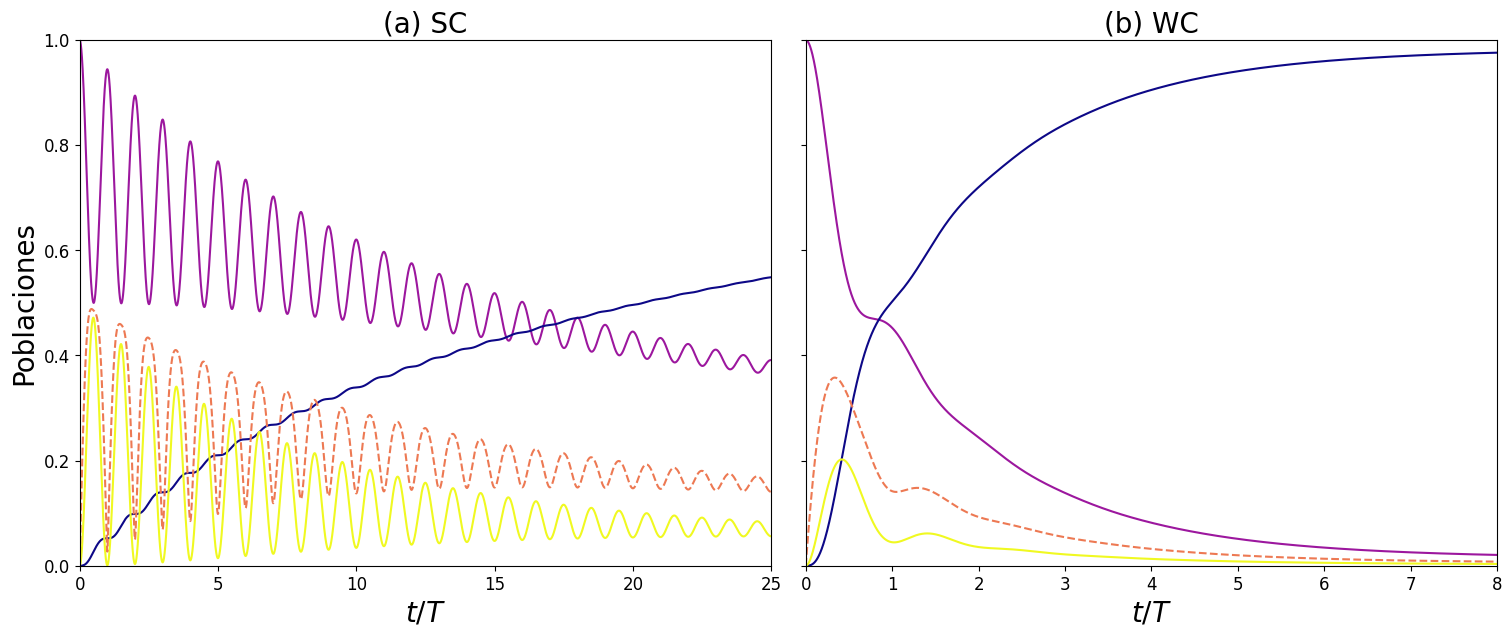
\includegraphics[width=\textwidth]{figuras/ch3/poblaciones sc vs wc.png}
    \caption{Solución númerica al sistema de ecuaciones dada por la ecuación de Lindblad para el estado inicial $\ket{e0}\bra{e0}$. Estos gráficos se realizaron con $\Delta=2g$; a la izquierda se observa el regimiento de Weak Coupling con $\gamma=0.1g$, donde el sistema átomo-cavidad esta debilmente acoplado con el entorno, y a la derecha el de Strong Coupling con $\gamma=2g$, donde las poblaciones y coherencias decaen sin oscilar. Las lineas solidas son las poblaciones de los estados, en azul para el estado $\ket{g0}$, en rojo para $\ket{e0}$ y en amarillo $\ket{g1}$, y la linea rayada representa la coherencia entre los estados con N=1 ($\ket{e0}$ y $\ket{g1}$). }
    \label{fig3:poblaciones e0}
\end{figure}

En el panel \ref{fig3:poblaciones e0}a, se muestra el regimen de SC, donde el acoplamiento entre el atomo y la cavidad es mayor al acomplamiento con el entorno, segun la relacion entre los parametros $\gamma/g=0.1$, y en el panel \ref{fig3:poblaciones e0}b, se muestra el caso del WK. La diferencia que es interesante para el problema, es que en el primer caso, tanto las poblaciones como las coherencias presentan oscilaciones coherentes antes de decaer por la influencia del entorno. En cambio, para el caso de WK, estas oscilaciones coherentes no estan presentes y el sistema llega a su estado asintotico en tiempos muy cortos. Las caracteristicas de la dinámica de cada regimen, influyen profundamente en el estudio de la fase geometrica, haciendo posible unicamente su utilizacion en el caso de Strong Coupling, donde la dinamica presenta oscilaciones coherentes durante varios ciclos, antes de decaer, haciendo del regimen de SC el unico escenario conveniente para su estudio. Antes de fundamentar esta afirmacion, se realiza un estudio poblacional en el caso de una cavidad con medio Kerr.

Como se vio anteriormente, el efecto del medio Kerr sobre los autoestados y las autoenergias es, por un lado, desplazar los niveles de energia.
\begin{figure}
    \centering
    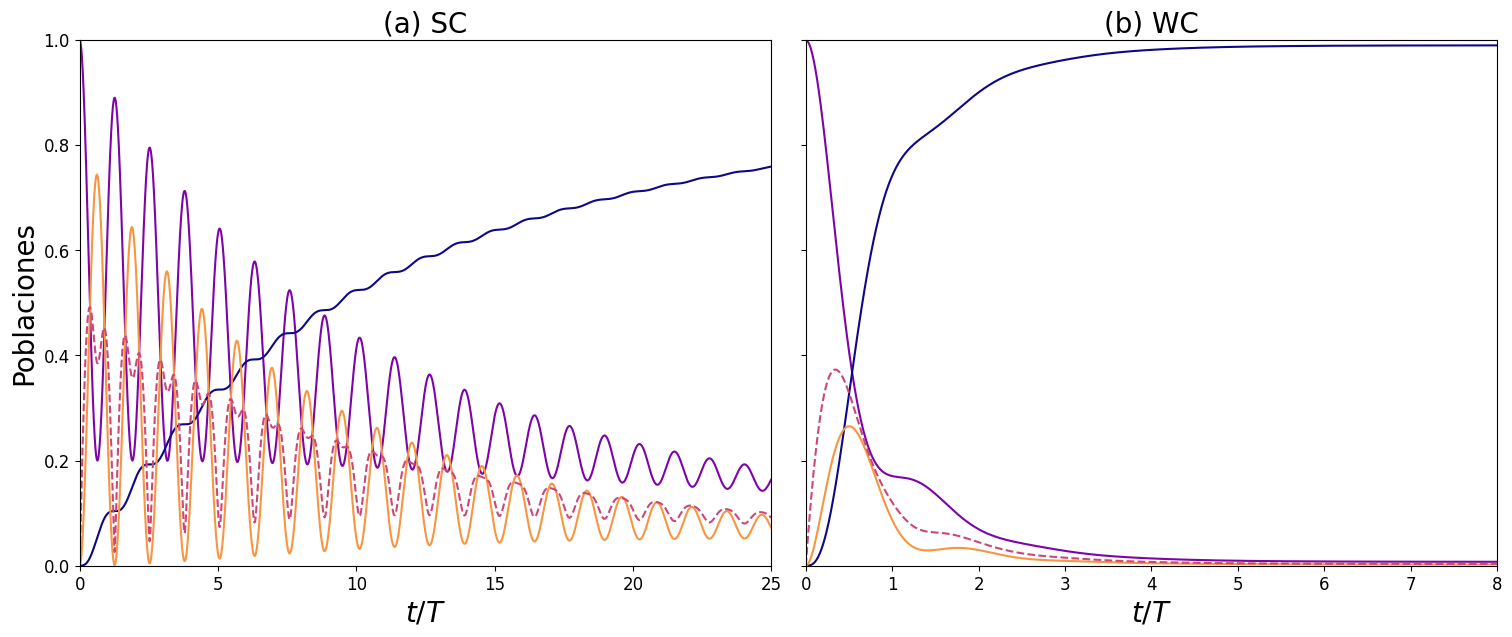
\includegraphics[width=\textwidth]{figuras/ch3/poblaciones kerr.png}
    \caption{Analisis poblacional para una cavidad con medio Kerr con $\chi=0.5g$.}
    \label{fig3:poblaciones kerr}
\end{figure}
Si se comparan las figuras \ref{fig3:poblaciones e0} con \ref{fig3:poblaciones kerr}, entonces se pueden observar dos diferencias. La primera es lo mencionado anteriormente; en el mismo tiempo, es decir entre $0\leq t/T \leq 25$, en el caso de $\chi=0$ se observan 25 oscilaciones, pero en el caso de $\chi=0.5g$ solo se observan 23 oscilaciones. Esto se debe a la condicion que se encontro al final de la seccion \ref{sec3:medio kerr}, en este caso se cumple que $\Delta=2g>(2n-1)\frac{\chi_1+\chi_2}{2}=1\cdot\frac{0.5g}{2}$, entonces la diferencia de energias entre los autoestados disminuye al aumentar $\chi$, y por lo tanto las oscilaciones son mas lentas para el caso de $\chi=0.5g$ en comparacion con $\chi=0$.

\subsection{Fase geometrica en presencia de disipación}
Ahora se estudia la fase geometrica adquirida por el sistema, calculada siguiendo la definicion \ref{}, y como esta se ve modificada con respecto del valor unitario por efecto del contacto con el entorno. Como el estado inicial es puro, la definicion se reduce al caso particular descripto por la ecuacion \ref{eq2}.

Los autovalores y autovectores del operador densidad pueden escribirse formalmente  diagonalizando el subespacio de 2x2 de la matriz densidad:
\begin{equation}
    \rho(t)=\begin{pmatrix}
        \rho_{00} & 0 & 0 & 0 &\dots \\
        0 & \rho_{11} & \rho_{12} & 0 & \dots \\
        0 & \rho_{21} & \rho_{22} & 0 & \dots \\ 
        \vdots & 0 & 0 & \ddots & \dots 
    \end{pmatrix}
\end{equation}
donde estamos nuevamente asumiendo una estructura diagonal por bloques, que se da cuando el estado inicial tiene un numero definido de escitaciones, dando lugar a dos autovectores. El de interes para utilizar la definicion de la fase geometrica \ref{}, es el autoestado
\begin{equation}
    \ket{\psi_+}(t)=\frac{-(\rho_{22}-\epsilon_+)\ket{e,0}+\rho_{21}\ket{g,1}}{\left((\rho_{22}-\epsilon_+)^2+\rho_{21}\rho_{12} \right)^{1/2}}
\end{equation}
con $\epsilon_+=\frac{1}{2}(\rho_{11}+\rho_{22}+((\rho_{11}-\rho_{22})^2+4\rho_{12}\rho_{21})^{1/2})$ el autovalor asociado. Recurriendo a este resultado, podemos escirbir formalmente la fase geometrica en funcion de los elementos de matriz $\rho_{ij}(t)$:
\begin{equation}
    \phi_g(t)=\int_0^t dt' \frac{\Im \dot\rho_{21}\rho_{12}}{(\rho_{22}-\epsilon_+)^2+\rho_{12}\rho_{21}}
\end{equation}

En general, esta fase diferirá de aquella acumulada en una evolución unitaria de forma que puede
escribirse, sin pérdida de generalidad, $\phi_g=\phi_u+\delta\phi$, con $\delta\phi$ la diferencia entre la fase unitaria y
aquella modificada por la presencia del entorno. Caracterizar la corrección $\delta\phi$ permite relacionar este
objeto, perteneciente a la geometría misma del espacio de Hilbert, con los efectos de disipación y
decoherencia experimentados por el sistema, así como determinar bajo qué circunstancias $\delta\phi$ resulta
despreciable y se puede considerar que la fase geométrica es robusta al efecto del entorno.

\subsubsection{Dependencia con el régimen de acoplamiento}

\subsubsection{Dependencia con el detunning}

\subsubsection{Dependencia con el medio Kerr}

\subsubsection{Robustez de la fase geométrica en el caso resonante}
